\documentclass{article}

\usepackage[polish]{babel}
\usepackage[utf8]{inputenc}
\usepackage{polski}
\usepackage[T1]{fontenc}
\usepackage{graphicx}

\graphicspath{ {./images/} }

\title{Klasyfikacja COVID-19 na zdjęciach rentgenowskich}
\author{Vladyslav Diachuk s18901}

\bibliographystyle{plain}

\makeindex
\begin{document}
\maketitle

%===================================================================================
\section{Wstęp}

%-----------------------------------------------------------------------------------
\subsection{Abstrakt}


%-----------------------------------------------------------------------------------
\subsection{Słowa kluczowe}


%-----------------------------------------------------------------------------------
\subsection{Teza główna}

%-----------------------------------------------------------------------------------
\subsection{Motywacja}


%===================================================================================
\section{Choroby płuc, rozpoznawanie, skutki}

%===================================================================================
\section{Uczenie maszynowe}
Uczeniem maszynowym nazywa się dziedzina nauki (i sztukę) programowania komputerów w sposób umożliwiający im uczenie się z danych \cite{geron} 
Ta praca jest zrobiona z użyciem uczenia maszynowego a zwłaszcza sieci neuronowych.


%===================================================================================
\section{Neuron}
Zanim opiszę sieci neuronowe, chcę przedstawić co to jest neuron (komórka).

\subsection{Neuron biologiczny}
Jak wiadomo mózg ludzki i większości innych organizmów składa się z malutkich komórek nerwowych, nazywanych neuron, zdolnych do przetwarzania i przewodzenia informacji w postaci sygnału elektrycznego. Neurony są podstawowym elementem układu nerwowego zwierząt. Najwięcej neuronów znajduje się w ośrodkowym układzie nerwowym, w skład którego wchodzi mózgowie oraz rdzeń kręgowy. \cite{neuroscience}
Głównymi elementami neuronu są ciało komórki zawierające jądro i większość organelli komórkowych, wiele rozgałęziających się wypustek zwanych dendrytami oraz jedna bardzo długa wypustka -- akson. \cite{geron}

\begin{figure}
	\centering
	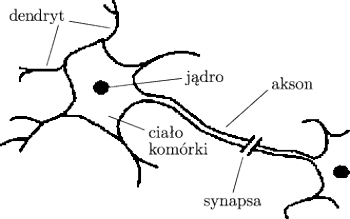
\includegraphics[width=\textwidth,height=6cm,keepaspectratio=true]{neuron_bio}
	\caption{
		Obraz komórki biologicznej \cite{neuron_bio}
	}
\end{figure}

Neurony biologiczne generują krótkie impulsy elektryczne zwane sygnałami, które są przenoszone wzdłuż aksonów i powodują uwalnianie w synapsach sygnałów chemicznych zwanych neuroprzekaźnikami. Kiedy komórka nerwowa otrzymuje dostateczną liczbę neuroprzekaźników od innych neuronów w ciągu kilku milisekund, to sama zaczyna wysyłać własne sygnały elektryczne (w rzeczywistości jest to uzależnione od neuroprzekaźników, gdyż niektóre z nich hamują aktywność komórki nerwowej). \cite{geron}
Zatem mechanizm działania poszczególnych neuronów jest dość prosty, tworzą one jednak rozległą sieć składającą się z miliardów komórek nerwowych, gdzie zazwyczaj jeden neuron łączy się z tysiącami innych. Dzięki tak olbrzymiej sieci zawierającej proste komórki nerwowe mogą być wykonywane skomplikowane obliczenia.

\subsection{Sztuczny neuron}
W 1943 przez Warren S. McCulloch i Walter Pitts było zaproponowano bardzo prostą reprezentację neuronu sztucznego. On ma co najmniej jedno binarne wejście i dokładnie jedno binarne wyjście. Wyjście zostanie aktywne tylko wtedy kiedy będzie aktywna określona liczba wejść. \cite{mcculloch1943logical} Tak prosty model daje nam bardzo duże możliwości. Twórcy udowodnili że za pomocą takich neuronów jesteśmy w stanie zaprotestować sieć która rozwiąże dowolne zadanie logiczne.

\begin{figure}
	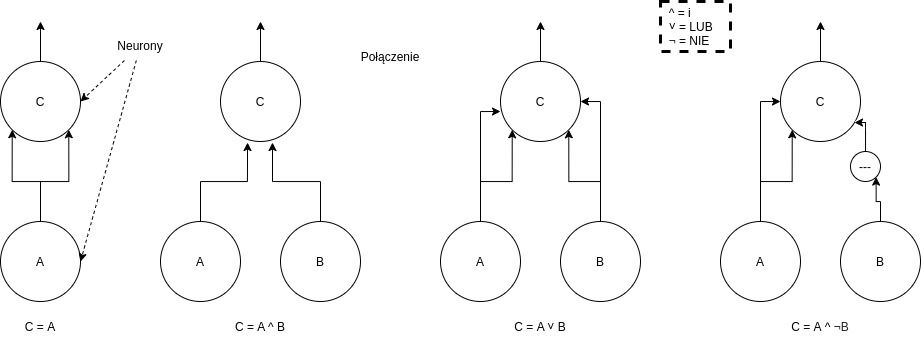
\includegraphics[width=\textwidth,keepaspectratio=true]{SSN_simple_neurons}
	\caption{
		Przykład sztucznych sieci neuronowych przeprowadzających proste operacje logiczne. Neuron aktywuje się przy co najmniej dwóch aktywnych wejściach \cite{geron}
	}
\end{figure}

Frank Rossenblatt trochę zmodyfikował ten neuron. 

Kluczowe zmiany:
\begin{itemize}
	\item Wartościami wejść/wyjść są liczby
	\item Każde połączenie ma przyporządkowaną wagę.
	\item Używanie funkcji skokowej na końcu
	\item Dodatkowe wejście z własną wagą, tak zwany bias
\end{itemize}

Jednostka wylicza ważoną sumę sygnałów wejściowych, a następnie zostaję użyta funkcja aktywacji

\begin{figure}
	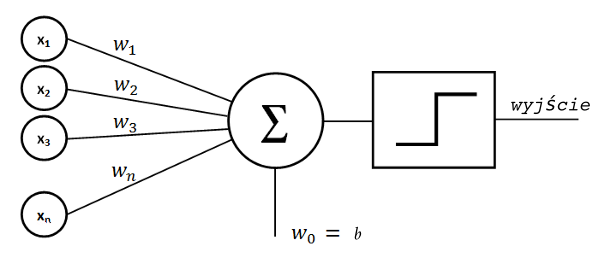
\includegraphics[width=\textwidth,keepaspectratio=true]{neuron_rosenblatta}
	\caption{
		Sztuczny neuron Franka Rosenblatta
	}
\end{figure}


%===================================================================================
\section{Sieci neuronowe w klasyfikacji danych wizualnych}

%-----------------------------------------------------------------------------------
\subsection{Model neuronu jako klasyfikator}

%-----------------------------------------------------------------------------------
\subsection{Konwolucyjne sieci neuronowe}

%-----------------------------------------------------------------------------------
\subsection{Uczenie sztucznych sieci neuronowych}



%===================================================================================
\section{Architektura konwolucyjna w detekcji chorób płuc}



\bibliography{bibliografia}

	
\end{document}